\documentclass[11pt]{beamer}
\usepackage[utf8]{inputenc}
\usepackage[english]{babel}
\usepackage{amsmath}
\usepackage{amsfonts}
\usepackage{amssymb}
\usepackage{graphicx}
\usepackage{longtable}
\usepackage{booktabs}
\usepackage[retainorgcmds]{IEEEtrantools}
\usepackage{subfigure}

% Pacotes para usar todonotes como default
\usepackage{xkeyval}
\usepackage{todonotes}
\presetkeys{todonotes}{inline}{}


\usetheme{AnnArbor}
\usecolortheme{beaver}
\begin{document}
\author{Marcelo Ruas e Alexandre Street}
\title{Scenario generation for nongaussian time series via Quantile Regression}
%\subtitle{}
	%\logo{}
	%\institute{}
	%\date{}
	%\subject{}
	%\setbeamercovered{transparent}
	%\setbeamertemplate{navigation symbols}{}
\begin{frame}[plain]
\maketitle
\end{frame}


\section{Introduction}\label{introduction}


\begin{frame}{Motivation}

	\begin{itemize}
		\item
		Renewable energy scenarios are important in many fields in Power
		Systems:
		
		\begin{enumerate}
			\def\labelenumi{\roman{enumi})}
			
			\item
			Energy trading;
			\item
			unit commitment;
			\item
			grid expansion planning;
			\item
			investment decisions
		\end{enumerate}
		\item
		In stochastic optimization problems, a set of scenarios is a needed
		input.
		\item
		Robust optimization requires bounds for probable values.
	\end{itemize}

	\textbf{Change in paradigm: from predicting the conditional mean to
		predicting the conditional distribution}

\end{frame}



\begin{frame}{Probability Forecasting Approaches}

	\begin{itemize}

	\item
	\emph{Parametric Models}

	\begin{itemize}
		
		\item
		Assume a distributional shape
		\item
		Low computational costs
		\item
		Faster convergence
		\item
		\emph{Examples: Arima-GARCH, GAS}
	\end{itemize}
	\item
	\emph{Nonparametric Models}

	\begin{itemize}
		
		\item
		Don't require a distribution to be specified
		\item
		High computational cost
		\item
		Needs more data to produce a good approximation

		\item Examples: Quantile Regression \cite{koenker1978regression}, Kernel Density Estimation \cite{gallego2016line} and Artificial Inteligende \cite{Wan2017}.
	\end{itemize}
	\end{itemize}

\end{frame}


\begin{frame}{Wind Power Time Series - Icaraizinho monthly data}

	\begin{figure}
	\centering
	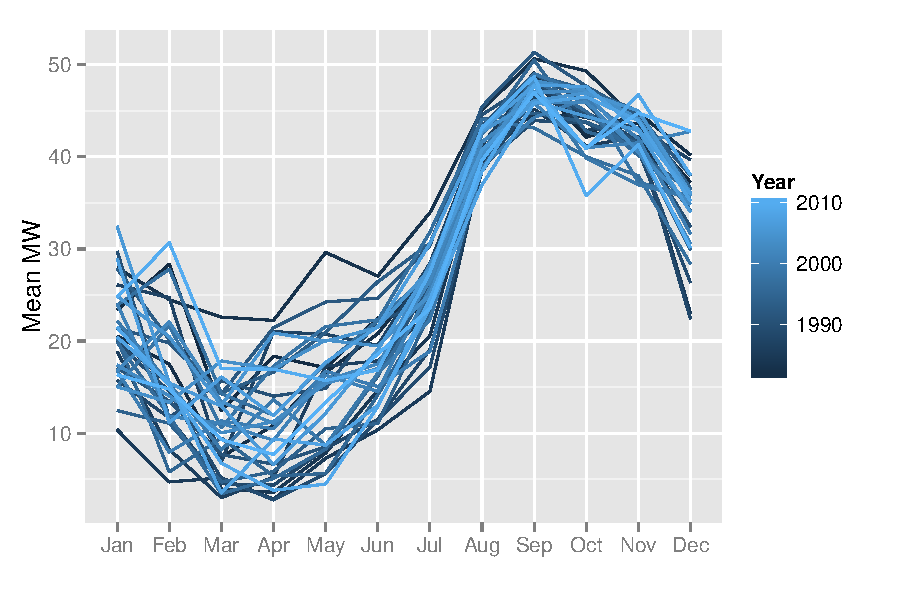
\includegraphics[width=0.9\linewidth]{Images/icaraizinho-mensal}
	\end{figure}

\end{frame}


\begin{frame}{Wind Power Time Series - Kaggle forecasting competition hourly data}

	\begin{figure}
	\centering
	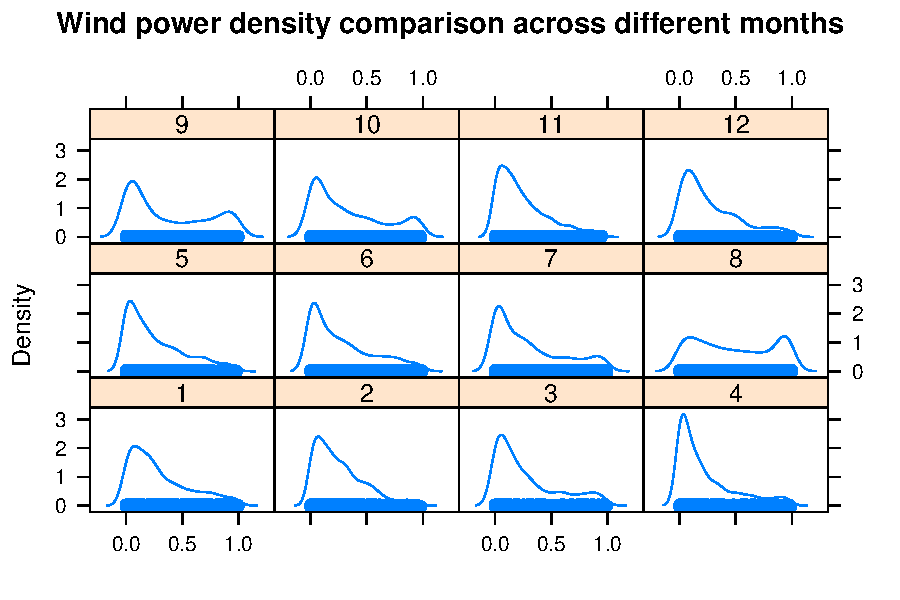
\includegraphics[width=0.9\linewidth]{Images/density}
	\end{figure}

\end{frame}

\begin{frame}{The nongaussianity of Wind Power}

	\begin{itemize}
	
	\item
	Renewables, such as wind and solar power have reportedly nongaussian behaviour.
	\item
	Convenience of using a nonparametric approach, which doesn't rely on assuming a distribution.
	\item
	Quantile regression is the chosen technique available to model this time series dynamics, by estimating a thin grid of $\alpha$-quantiles at once and forming a data-driven conditional distribution
	\end{itemize}
	
\end{frame}


\begin{frame}{Scenario Simulation}

	\begin{itemize}
		\item In order to simulate scenarios, not only the conditional mean is needed, but the whole conditional distribution, whose estimation procedure is the most important contribution in this work.
		
		\item The procedure is drawing, in each period $\tau$, a value for $\tau+1$ from the estimated conditional distribution function (CDF). Hence, having a good estimate of the CDF is essential to meet the goal in this work. 

		\todo{Put a simulation graph}

	\end{itemize}
\end{frame}



\begin{frame}{Building an estimator of the CDF}
	\begin{itemize}
		\item Construct the CDF nonparametrically by using a sequence of quantile values $q_\alpha$ by estimating many quantiles on a thin grid of probabilities over the interval $[0,1]$. 
		
		\item Transforming this set of points $q_{\alpha_1}, q_{\alpha_2}, \dots, q_{\alpha_{|J|}}$ into a continuous function by using a interpolating method. 

		\todo{Picture with points}
	\end{itemize}
	% These quantile values may be estimated by a technique such as Quantile Regression (QR). 
	% The seminal work \cite{koenker1978regression} defines QR as it is employed in many works \cite{chao_quantile_2012,li_quantile_2007,bosch_convergent_nodate,gallego2016line,moller_time-adaptive_2008,nielsen2006,bremnes_probabilistic_2004,wan_direct_2017}. The conditional quantile is the solution of an optimization problem where the sum of the check function (defined formally in the next session) is minimized. Instead of using the classical regression to estimate the conditional mean, QR determines any quantile from the conditional distribution. Applications are enormous, ranging from risk measuring at financial funds (the Value-at-Risk) to a central measure robust to outliers.
\end{frame}


\begin{frame}{Quantile Regression}
	\begin{itemize}
		\item Defined by \cite{koenker1978regression} as the solution of the following minimization problem 
			\begin{equation}
				\underset{q\in\mathcal{Q}}{\text{min}}\, L_\alpha(q) = \sum_{t\in T}\rho_{\alpha}(y_{t}-q(x_t)),\label{eq:optim-lqr1} 
			\end{equation}
			where
			\begin{equation}\label{eq:check-function}
				\rho_{\alpha}(x)=\begin{cases}
				\alpha x & \text{if }x\geq0\\
				(1-\alpha)x & \text{if }x<0
				\end{cases}.
			\end{equation}
	\end{itemize}
\end{frame}


\begin{frame}{QR to model Wind Power Time Series}
	\begin{itemize}
		\item \cite{moller_time-adaptive_2008}: updating quantile regression model.
		\item \cite{nielsen2006}: builds a quantile model using already existent independent forecasts.
		\item \cite{gallego-castillo_-line_2016}: uses nonparametric QR with a Reproducing Kernel Hilbert Space.
		\item \cite{wan2016}: Neural network with one hidden layer (extreme learning machine) to forecast quantiles.
	\end{itemize}
\end{frame}

\begin{frame}{Blau}
\begin{figure}
\begin{center}
	\includegraphics[width=0.7\linewidth,height=0.7\textheight,keepaspectratio]{pg_0004}
\end{center}
\caption{ADA}
\end{figure}
\end{frame}

\begin{frame}{Blau2}
	\begin{figure}
	\begin{center}
		\includegraphics[width=0.7\textwidth]{pg_0004}
	\end{center}
	\caption{eki}
	\end{figure}
\end{frame}
	


\begin{frame}{Proposed methodology to estimate the Conditional Density Function}
\begin{figure}
\begin{center}
	\includegraphics[width=0.75\textwidth]{Images/Diagrama-trabalho}
\end{center}
\end{figure}
\end{frame}






\begin{frame}{Objectives}
	\begin{itemize}
		\item A nonparametric methodology to model, from a set of quantile estimations, the conditional distribution of RG time series to produce future scenarios.
		
		\item The proposition of two different procedures to jointly estimate quantiles: (i) A linear model that selects the global optimal solution with parsimony both on the selection of covariates as on the quantiles. This methodology is based on the Adaptive LASSO for QR (Linear Programming). (ii) A nonparametric quantile regression model, which has a free functional form, tuned by a penalty on how rough this function may be. 
		
		\item Regularization techniques applied to an ensemble of quantile functions to estimate the conditional distribution, solving the issue of non-crossing quantiles. On regularizing quantiles, we propose a smoothness on the coefficient value across the sequence of quantiles.
		%\item A nonlinear QR
		
	\end{itemize}
	
\end{frame}




% \section{Quantile Regression}\label{quantile-regression}

\begin{frame}{Definition of the Conditional Quantile}


\begin{columns}

\column{0.5\textwidth}

\tiny

Let the conditional quantile function of \(Y\) for a given value \(x\)
of the \(d\)-dimensional random variable \(X\), i.e.,
\(Q_{Y|X}:[0,1] \times \mathbb{R}^d \rightarrow \mathbb{R}\), can be
defined as:
\[Q_{Y|X}(\alpha,x) = F_{Y|X=x}^{-1}(\alpha) = \inf\{y: F_{Y|X=x}(y) \geq \alpha\}.\]

\begin{block}{Quantile function for a finite sample $\{ y_t,x_t \}_{t \in T}$}
    \begin{equation*}
        \hat{Q}_{Y|X}(\alpha,\cdot)\quad\in\quad  \underset{q\in\mathcal{Q}}{\text{arg min}}\, L_\alpha(q) = \sum_{t\in T}\rho_{\alpha}(y_{t}-q(x_t))
    \end{equation*}
    $$
    \rho_{\alpha}(x)=\begin{cases}
        \alpha x & \text{if }x\geq0\\
        (1-\alpha)x & \text{if }x<0
        \end{cases}
    $$
\end{block}

\column{0.5\textwidth}

\end{columns}

\end{frame}

% \begin{frame}{Conditional Quantile from a sample}

% Let a dataset be composed from \(\{y_t,x_t \}_{t \in T}\) and let
% \(\rho\) be the check function

% \begin{equation}\label{eq:check-function}
% \rho_{\alpha}(x)=\begin{cases}
% \alpha x & \text{if }x\geq0\\
% (1-\alpha)x & \text{if }x<0
% \end{cases},
% \end{equation}

% The sample quantile function for a given probability \(\alpha\) is then
% based on a finite number of observations and is the solution to
% minimizing the loss function \(L(\cdot)\): \[
% \hat{Q}_{Y|X}(\alpha,\cdot)\quad\in\quad  \underset{q(\cdot)\in\mathcal{Q}}{\text{arg min}}\, L_\alpha(q) = \sum_{t\in T}\rho_{\alpha}(y_{t}-q(x_t)), 
% \] \[
% q(x_t) = \beta_0 + \beta^T x_t,
% \] where \(\mathcal{Q}\) is a space of functions. In this paper, we use
% \(\mathcal{Q}\) as an \textbf{affine functions space}.

% \end{frame}

% \begin{frame}{Conditional Quantile from a sample}

% \begin{itemize}

% \item
% For a single quantile, this problem can be solved by the following
% Linear Programming problem: \[
% \begin{array}{lll}
% \underset{\beta_0, \beta,\varepsilon_{t}^{+}, \varepsilon_{t}^{-}}{\text{min}} & \sum_{t \in T} \left(\alpha \varepsilon_{t}^{+}+(1-\alpha)\varepsilon_{t}^{-}\right) & \\
% \mbox{s.t. } & \varepsilon_{t}^{+}-\varepsilon_{t}^{-}=y_{t} - \beta_{0} - \beta^T x_{t}, & \qquad\forall t \in T,\\
% & \varepsilon_t^+,\varepsilon_t^- \geq 0, & \qquad \forall t \in T.
% \end{array}
% \]
% \item
% The output are the coefficients \(\beta_0\) and \(\beta\) (which is
% the same dimension as \(x_t\)), that describe the quantile function as
% an affine function.
% \end{itemize}

% \end{frame}

% \begin{frame}{The non-crossing issue}

% \begin{itemize}
% 	\item The following condition must always hold:
% 	$$q_\alpha(x_t) \leq q_{\alpha'}(x_t) \text{, when } \alpha \leq \alpha'$$
% \end{itemize}

% \begin{figure}
% \centering
% \begin{minipage}[t]{\linewidth}
% \centering
% \begin{minipage}[t]{0.45\linewidth}
% \centering     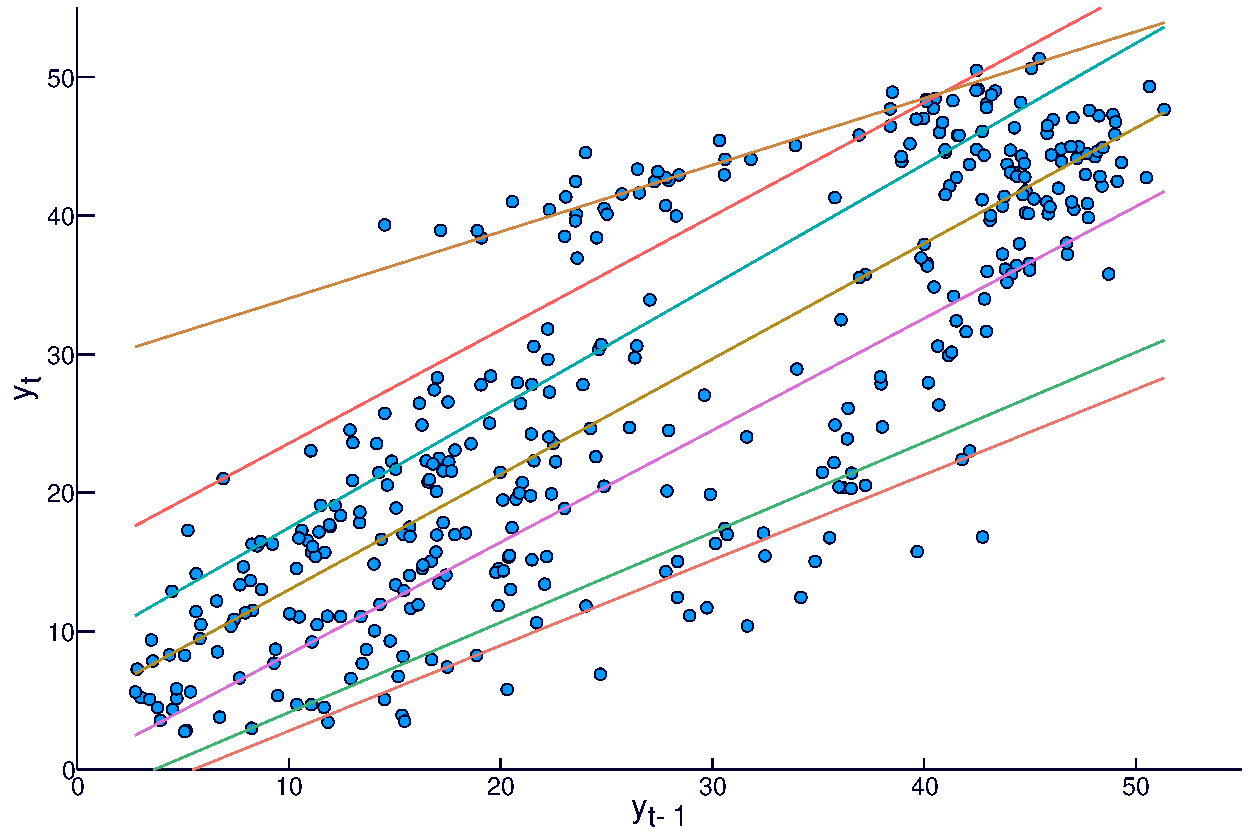
\includegraphics[width=\textwidth]{Images/icaraizinho-quantile-linear-scatter-crossing}
% \subcaption{Each $\alpha$-quantile estimated independently}
% \end{minipage}
% \begin{minipage}[t]{0.45\linewidth}
% \centering     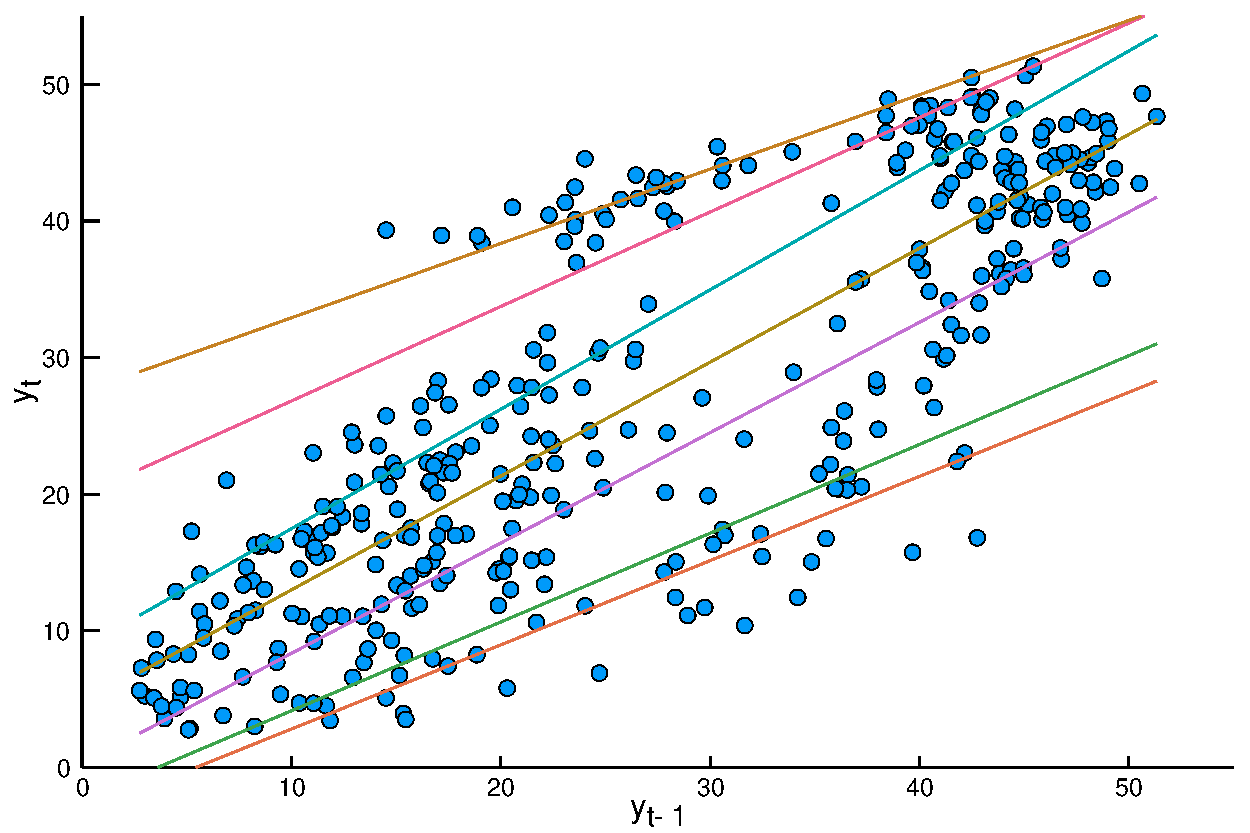
\includegraphics[width=\textwidth]{Images/icaraizinho-quantile-linear-scatter}
% \subcaption{Estimation with non-crossing constraint}
% \end{minipage}
% \end{minipage}
% \caption{These graphs show how the addition of a constraint can contour the crossing quantile issue}
% \label{fig:quantiles-vs-xt}
% \end{figure}

% \end{frame}

% \begin{frame}{Notation}

% \small

% \begin{longtable}[]{@{}ll@{}}
% \toprule
% \begin{minipage}[b]{0.14\columnwidth}\raggedright\strut
% Expression\strut
% \end{minipage} & \begin{minipage}[b]{0.80\columnwidth}\raggedright\strut
% Meaning\strut
% \end{minipage}\tabularnewline
% \midrule
% \endhead
% \begin{minipage}[t]{0.14\columnwidth}\raggedright\strut
% \(Q_{Y \mid X}(\alpha,x)\)\strut
% \end{minipage} & \begin{minipage}[t]{0.80\columnwidth}\raggedright\strut
% The conditional quantile function\strut
% \end{minipage}\tabularnewline
% \begin{minipage}[t]{0.14\columnwidth}\raggedright\strut
% \(y_t\)\strut
% \end{minipage} & \begin{minipage}[t]{0.80\columnwidth}\raggedright\strut
% the time series we are modelling\strut
% \end{minipage}\tabularnewline
% \begin{minipage}[t]{0.14\columnwidth}\raggedright\strut
% \(x_t\)\strut
% \end{minipage} & \begin{minipage}[t]{0.80\columnwidth}\raggedright\strut
% explanatory variables of \(y_t\) in \(t\)\strut
% \end{minipage}\tabularnewline
% \begin{minipage}[t]{0.14\columnwidth}\raggedright\strut
% \(T\)\strut
% \end{minipage} & \begin{minipage}[t]{0.80\columnwidth}\raggedright\strut
% the set containing all observations indexes\strut
% \end{minipage}\tabularnewline
% \begin{minipage}[t]{0.14\columnwidth}\raggedright\strut
% \(J\)\strut
% \end{minipage} & \begin{minipage}[t]{0.80\columnwidth}\raggedright\strut
% the set containing all quantile indexes\strut
% \end{minipage}\tabularnewline
% \begin{minipage}[t]{0.14\columnwidth}\raggedright\strut
% \(J_{(-1)}\)\strut
% \end{minipage} & \begin{minipage}[t]{0.80\columnwidth}\raggedright\strut
% the set \(J\backslash \{1\}\)\strut
% \end{minipage}\tabularnewline
% \begin{minipage}[t]{0.14\columnwidth}\raggedright\strut
% \(\alpha_j\)\strut
% \end{minipage} & \begin{minipage}[t]{0.80\columnwidth}\raggedright\strut
% a probability, might be indexed by \(j\)\strut
% \end{minipage}\tabularnewline
% \begin{minipage}[t]{0.14\columnwidth}\raggedright\strut
% \(A\)\strut
% \end{minipage} & \begin{minipage}[t]{0.80\columnwidth}\raggedright\strut
% the set of probabilities \(\{\alpha_j \mid j \in J\}\)\strut
% \end{minipage}\tabularnewline
% \begin{minipage}[t]{0.14\columnwidth}\raggedright\strut
% \(K\)\strut
% \end{minipage} & \begin{minipage}[t]{0.80\columnwidth}\raggedright\strut
% Maximum number of covariates on MILP regularization\strut
% \end{minipage}\tabularnewline
% \begin{minipage}[t]{0.14\columnwidth}\raggedright\strut
% \(\lambda\)\strut
% \end{minipage} & \begin{minipage}[t]{0.80\columnwidth}\raggedright\strut
% The Lasso penalization on the coefficients \(\ell_1\)-norm\strut
% \end{minipage}\tabularnewline
% \begin{minipage}[t]{0.14\columnwidth}\raggedright\strut
% \(\gamma\)\strut
% \end{minipage} & \begin{minipage}[t]{0.80\columnwidth}\raggedright\strut
% The penalization on the coefficients second-derivative with respect of
% the quantiles\strut
% \end{minipage}\tabularnewline
% \bottomrule
% \end{longtable}

% \end{frame}

% \begin{frame}{Conditional Quantile as a Linear Programming Problem}

% \[
% \min_{\beta_{0j},\beta_j,\varepsilon_{tj}^{+}, \varepsilon_{tj}^{-}} \, \sum_{j \in J} \sum_{t \in T}\left(\alpha_j \varepsilon_{t j}^{+}+(1-\alpha_j)\varepsilon_{t j}^{-}\right)
% \] \[
% \begin{array}{lr}
% \text{s.t.} &\\
% \varepsilon_{t j}^{+}-\varepsilon_{t j}^{-}=y_{t} - \beta_{0j} - \beta_{j}^T x_{t}, & \forall t \in T, \forall j \in J, \\
% \varepsilon_{tj}^+,\varepsilon_{tj}^- \geq 0, & \forall t \in T,\forall j \in J,\\
% \beta_{0,j-1} + \beta_{j-1}^T x_{t} \leq \beta_{0j} + \beta_{j}^T x_{t},
% & \forall t \in T, \forall j \in J_{(-1)},
% \end{array}
% \]

% \begin{itemize}
% \item
% Coefficients \(\beta_{0j}\) and \(\beta_j\) refer to the
% \(j\)\textsuperscript{th} quantile
% \item
% We apply QR to estimate the conditional distribution
% \(\hat{Q}_{Y_{t+h}|X_{t+h},Y_t, Y_{t-1}, \dots} (\alpha,\cdot)\) for a
% \(k\)-step ahead forecast of time serie \(\{y_t\}\), where \(X_{t+h}\)
% is a vector of exogenous variables at the time we want to forecast.
% \end{itemize}

% \end{frame}

% \section{Regularization of
% covariates}\label{regularization-of-covariates}

% \begin{frame}{Best Subset selection via MILP}

% \begin{itemize}

% \item
% Mixed Integer Linear Programming (MILP) models allow only \(K\)
% variables to be used for each \(\alpha\)-quantile.
% \item
% Only \(K\) coefficients \(\beta_{pj}\) may have nonzero values, for
% each \(\alpha\)-quantile.
% \item
% It is guaranteed by constraints on the optimization model.
% \item
% One model for each \(\alpha\)-quantile
% \end{itemize}

% \end{frame}

% \begin{frame}{Best Subset selection via MILP}


% \begin{IEEEeqnarray*}{llr}
% \underset{\beta_{0j},\beta_j,z_{p j}, \varepsilon_{t j}^{+},\varepsilon_{t j}^{-}}{\text{min}} & \sum_{j \in J} \sum_{t\in T}\left(\alpha_j\varepsilon_{t j}^{+}+(1-\alpha_j)\varepsilon_{t j}^{-}\right)  & \\
% \mbox{s.t } & \varepsilon_{t j}^{+}-\varepsilon_{t j}^{-}=y_{t}-\beta_{0 j}-\beta_{j}^T x_{t},& \forall t \in T ,\forall j \in J, \\
% & \varepsilon_{t j}^{+},\varepsilon_{t j}^{-}\geq0,&\forall t \in T ,\forall j \in J, \\
% & - M z_{p j} \leq \beta_{p j} \leq M z_{p j},& \forall j \in J, \forall p\in P, \\
% & \sum_{p \in P} z_{p j} \leq K, &  \forall j \in J, \\
% & z_{p j} \in \{0,1\},& \forall j \in J, \forall p\in P,\\
% & \beta_{0,j-1} + \beta_{j-1}^T x_{t} \leq \beta_{0j} + \beta_{j}^T x_{t}, & \quad \forall t \in T, \forall j \in J_{(-1)},
% \end{IEEEeqnarray*}


% \begin{itemize}

% \item
% \(z_{pj}\) is a binary variable which indicates when
% \(\beta_{pj} > 0\).
% \end{itemize}

% \end{frame}

% \begin{frame}{Variable Selection via LASSO}

% \begin{itemize}

% \item
% Regularization by including the coefficients \(\ell_1\)-norm on the
% objective function.
% \item
% In this method, coefficients are shrunk towards zero by changing a
% continuous parameter \(\lambda\), which penalizes the size of the
% \(\ell_1\)-norm.\\
% \item
% When the value of \(\lambda\) gets bigger, fewer variables are
% selected to be used.
% \item
% The optimization problem for a single quantile is presented below: 
% \[
% \underset{\beta_{0},\beta}{\text{min}} \sum_{t\in T}\rho_{\alpha}(y_{t}-(\beta_0 + \beta^T x_t))+\lambda\|\beta\|_{1},
% \]
% \end{itemize}

% \end{frame}

% \begin{frame}{Variable Selection via LASSO}

% \begin{itemize}

% \item
% At first, we select variables using LASSO
% \end{itemize}

% \begin{IEEEeqnarray*}{lr}
% \underset{\beta_{0},\beta,\varepsilon_{t j}^{+},\varepsilon_{t j}^{-}}{\text{arg min}} \sum_{j \in J} \sum_{t \in T}\left(\alpha_j \varepsilon_{t j}^{+}+(1-\alpha_j)\varepsilon_{t j}^{-}\right)+\lambda\sum_{p \in P}\mbox{\ensuremath{\xi}}_{p j} \span \label{eq:obj-lasso} \\
% \mbox{subject to} \span \\
% \varepsilon_{t j}^{+}-\varepsilon_{t j}^{-}= y_{t}-\beta_{0 j}-\beta_{j}^T x_{t},&\forall t\in T, \forall j \in J, \\
% \varepsilon_{t j}^{+},\varepsilon_{t j}^{-}\geq0,&\forall t \in T, \forall j \in J,\\
% \xi_{p\alpha}\geq\beta_{p j},&\forall p\in P, \forall j \in J, 
% \\
% \xi_{p\alpha}\geq-\beta_{p j},&\forall p\in P, \forall j \in J\\
% \beta_{0,j-1} + \beta_{j-1}^T x_{t} \leq \beta_{0j} + \beta_{j}^T x_{t}, & \quad \forall t \in T, \forall j \in J_{(-1)},\\
% \end{IEEEeqnarray*}

% \end{frame}

% \begin{frame}{Variable Selection via LASSO}

% \begin{itemize}
% \item
% We then define \(S_\lambda\) as the set of indexes of selected
% variables given by \[
% S_{\lambda} = \{ p \in \{ 1,\dots,P \} | \; |\beta^{*LASSO}_{\lambda,p}| \neq 0  \}.
% \] Hence, we have that, for each \(p \in \{ 1,\dots,P \}\),
% \[\beta^{*LASSO}_{\theta,p} = 0 \Longrightarrow \beta^{*}_{\theta,p} = 0.\]
% \item
% On the second stage, we estimate coefficients using a regular QR where
% input variables are only the ones which belonging to \(S_\lambda\)
% \end{itemize}

% \end{frame}

% \section{Regularization on the
% quantiles}\label{regularization-on-the-quantiles}

% \begin{frame}{Regularization on the quantiles - Motivation}
% 	In practice, often when we regularize 
% 	\begin{figure}
% 		\centering
% 		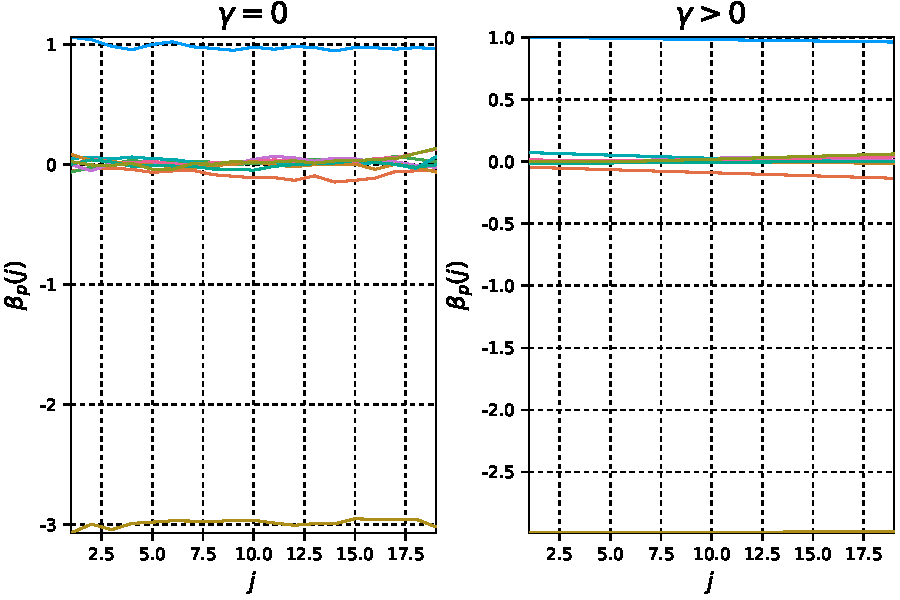
\includegraphics[width=0.5\linewidth]{Images/Lambda10-gamma03.pdf}
% 	\end{figure}
	
% \end{frame}


% \begin{frame}{MILP - Defining groups for \(\alpha\)-quantiles}


% \begin{IEEEeqnarray*}{lll}
% \underset{\beta_{0j},\beta_j,z_{p j}, \varepsilon_{t j}^{+},\varepsilon_{t j}^{-}}{\text{min}} & \sum_{j \in J} \sum_{t\in T}\left(\alpha_j\varepsilon_{t j}^{+}+(1-\alpha_j)\varepsilon_{t j}^{-}\right)  & \\
% \mbox{s.t } & \varepsilon_{t j}^{+}-\varepsilon_{t j}^{-}=y_{t}-\beta_{0 j}-\beta_{j}^T x_{t},& \forall t \in T ,\forall j \in J, \\
% & \varepsilon_{t j}^{+},\varepsilon_{t j}^{-}\geq0,&\forall t \in T ,\forall j \in 
% J, \\
% &\mathcal{Z}_{p j g} := 2 - ( 1-z_{pg}) - I_{gj}, & \\
% & - M \mathcal{Z}_{p j g} \leq \beta_{p j} \leq M \mathcal{Z}_{p j g},& \forall j \in J, \forall p\in P, \forall g \in G   \\
% & \sum_{p \in P} z_{p g} \leq K, &  \forall j \in J, \\
% & \beta_{0,j-1} + \beta_{j-1}^T x_{t} \leq \beta_{0j} + \beta_{j}^T x_{t}, & \forall t \in T, \forall j \in J_{(-1)},\\
% & I_{gj}, z_{pg} \in \{0,1\},& \forall p \in P,\forall g \in G, \\
% & z_{p g} \in \{0,1\},& \forall j \in J, \forall p\in P,\\
% \end{IEEEeqnarray*}


% \end{frame}




% \begin{frame}{MILP with quantile regularization}

% \small
% \begin{IEEEeqnarray*}{lr}
% 	\underset{\beta_{0j},\beta_j,z_{p j} \varepsilon_{t j}^{+},\varepsilon_{t j}^{-}}{\text{min}} \sum_{j \in J} \sum_{t\in T}\left(\alpha_j\varepsilon_{t j}^{+}+(1-\alpha_j)\varepsilon_{tj}^{-}\right) \nonumber \span \\
% 	\span + \gamma \sum_{j \in J'} (D2_{pj}^+ + D2_{pj}^-)   \\
% 	\mbox{subject to} \span \nonumber \\
% 	\varepsilon_{t j}^{+}-\varepsilon_{t j}^{-}=y_{t}-\beta_{0 j}-\beta_{j}^T x_{t,p},& \forall t \in T ,\forall j \in J,\\
% 	- M z_{p \alpha} \leq \beta_{p j} \leq M z_{p \alpha}, & \forall j \in J, \forall p\in P, \\
% 	\sum_{p \in P} z_{p \alpha} \leq K, & \forall j \in J, \\
% 	D2_{pj}^+ - D2_{pj}^- = \frac{\left(\frac{\beta_{p,j+1}-\beta_{pj}}{\alpha_{j+1}-\alpha_{j}}\right)-\left(\frac{\beta_{p,j}-\beta_{p,j-1}}{\alpha_{j}-\alpha_{j-1}}\right)}{\alpha_{j+1}-2\alpha_{j}+\alpha_{j-1}}, \span   \nonumber \\
% 	\span \forall j \in J_{(-1)}, \forall p\in P, \\
% 	\beta_{0j} + \beta_{j}^T x_{t} \leq \beta_{0,j+1} + \beta_{j+1}^T x_{t},&\forall t \in T, \forall j \in J_{(-1)}, \\
% 	z_{p \alpha} \in \{0,1\}, & \forall j \in J,  \forall p\in P, \\
% 	\varepsilon_{t j}^{+},\varepsilon_{t j}^{-}\geq0, & \forall t \in T ,\forall j \in J, \\
% 	D2_{pj}^+, D2_{pj}^- \geq 0, & \forall j \in J,  \forall p\in P.
% \end{IEEEeqnarray*}

% \end{frame}

% \begin{frame}{LASSO with quantile regularization}
% \footnotesize
% \begin{IEEEeqnarray*}{lr}
% 	\tilde \beta_\lambda^{*LASSO} = \underset{\beta_{0},\beta,\varepsilon_{t j}^{+},\varepsilon_{t j}^{-}}{\text{arg min}} \sum_{j \in J} \sum_{t \in T}(\alpha_j\varepsilon_{t j}^{+}+(1-\alpha_j)\varepsilon_{t j}^{-}) \span \nonumber \\
% 	\span +\lambda\sum_{p \in P}\mbox{\ensuremath{\xi}}_{p j} + \gamma \sum_{j \in J'} (D2_{pj}^+ + D2_{pj}^-)  \label{eq:obj-lasso} \\
% 	\mbox{subject to } \nonumber & \\
% 	\varepsilon_{t j}^{+}-\varepsilon_{t j}^{-}=y_{t}-\beta_{0 j}-\beta_{j}^T x_{t,p},& \forall t \in T ,\forall j \in J,\\
% 	\xi_{pj}\geq\beta_{p j},&\forall p\in P, \forall j \in J,  \label{l1-qar-3}
% 	\\
% 	\xi_{pj}\geq - \beta_{p j},&\forall p\in P, \forall j \in J,  \label{l1-qar-4}
% 	\\
% 	D2_{pj}^+ - D2_{pj}^- = \frac{\left(\frac{\beta_{p,j+1}-\beta_{pj}}{\alpha_{j+1}-\alpha_{j}}\right)-\left(\frac{\beta_{p,j}-\beta_{p,j-1}}{\alpha_{j}-\alpha_{j-1}}\right)}{\alpha_{j+1}-2\alpha_{j}+\alpha_{j-1}}, \span   \nonumber \\
% 	\span \forall j \in J_{(-1)}, \forall p\in P, \\
% 	\beta_{0j} + \beta_{j}^T x_{t} \leq \beta_{0,j+1} + \beta_{j+1}^T x_{t},&\forall t \in T, \forall j \in J_{(-1)}, \\
% 	\varepsilon_{t j}^{+},\varepsilon_{t j}^{-}\geq0,&\forall t \in T, \forall j \in J,\\
% 	D2_{pj}^+, D2_{pj}^- \geq 0, & \forall j \in J,  \forall p\in P. \label{eq:l1-qar5} 
% \end{IEEEeqnarray*}


% %
% %\begin{eqnarray*}
% %\underset{\beta_{0},\beta,\varepsilon_{t j}^{+},\varepsilon_{t j}^{-}}{\text{arg min}} & \sum_{j \in J} \sum_{t \in T}\left(\alpha_j \varepsilon_{t j}^{+}+(1-\alpha_j)\varepsilon_{t j}^{-}\right)+\lambda\sum_{p=1}^{P}\mbox{\ensuremath{\xi}}_{p j} + \gamma \sum_{j \in J'} D2_{pj} \span \label{eq:obj-lasso} \\
% %\mbox{s.t. } & \varepsilon_{t j}^{+}-\varepsilon_{t j}^{-}= y_{t}-\beta_{0 j}-\sum_{p=1}^{P}\beta_{p j}\tilde x_{t,p},&\forall t\in T, \forall j \in J, \\
% %& \varepsilon_{t j}^{+},\varepsilon_{t j}^{-}\geq0,&\forall t \in T, \forall j \in J,\\
% %& \xi_{p\alpha}\geq\beta_{p j},&\forall p\in P, \forall j \in J,  \label{l1-qar-3}
% %\\
% %& \tilde{D}_{pj}^{2}=\frac{\left(\frac{\beta_{p,j+1}-\beta_{pj}}{\alpha_{j+1}-\alpha_{j}}\right)-\left(\frac{\beta_{p,j}-\beta_{p,j-1}}{\alpha_{J}-\alpha_{j-1}}\right)}{\alpha_{j+1}-2\alpha_{j}+\alpha_{j-1}} \span\\
% %& D2_{pj} >  \tilde D_{pj}^{2} &  \forall j \in J_{(-1)}, \forall p\in P, \\
% %& D2_{pj} >  - \tilde D_{pj}^{2} &  \forall j \in J_{(-1)}, \forall p\in P,\\
% %& \beta_{0,j-1} + \beta_{j-1}^T x_{t} \leq \beta_{0j} + \beta_{j}^T x_{t}, & \forall t \in T, \forall j \in J_{(-1)},\\
% %& \xi_{pj}\geq-\beta_{p j},&\forall p\in P, \forall j \in J. 
% %\end{eqnarray*}

% \end{frame}

% \begin{frame}{Regularization on the quantiles}

% %\begin{figure}
% %\centering
% %\includegraphics[width=0.9\linewidth]{Images/}
% %\end{figure}

% \end{frame}

% \begin{frame}{LASSO - Penalization of derivative}

% \begin{figure}
% \centering
% 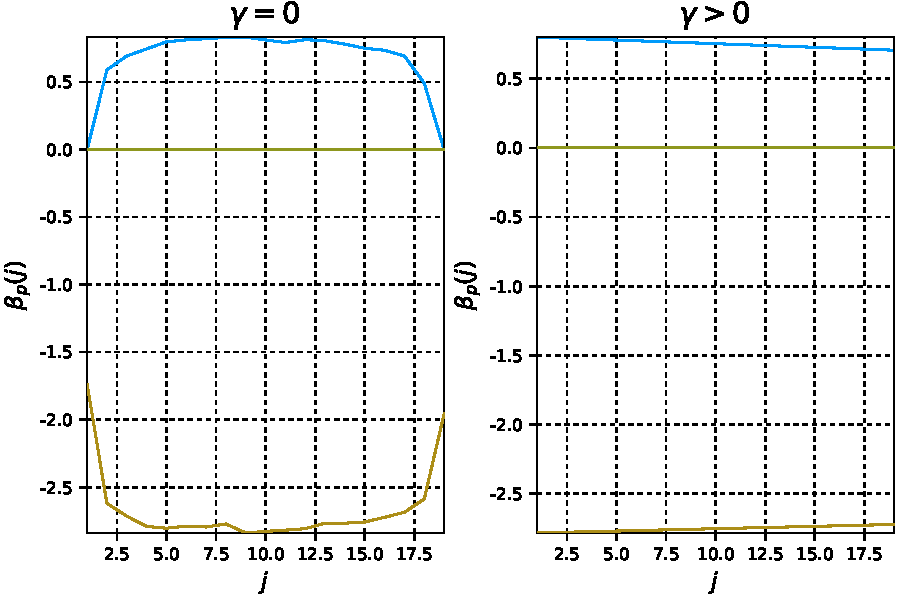
\includegraphics[width=0.9\linewidth]{Images/Lambda500-gamma30.pdf}
% \end{figure}

% \end{frame}

% \begin{frame}{LASSO - Penalization of derivative}

% \begin{figure}
% \centering
% 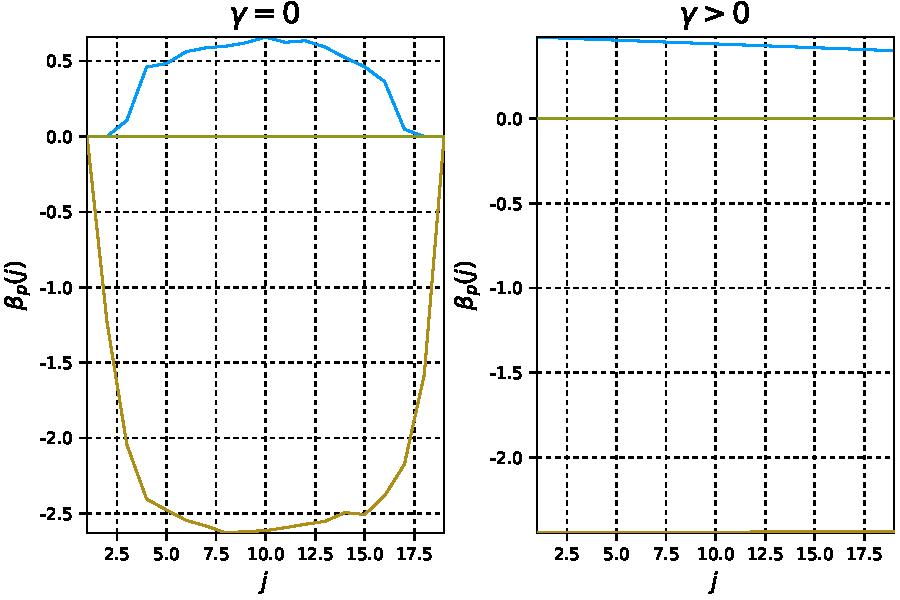
\includegraphics[width=0.7\linewidth]{Images/Lambda1000-gamma100.pdf}
% \caption{Testing caption}
% \end{figure}

% \end{frame}


% \begin{frame}{ADALASSO}

% \small
% LASSO solutions are solutions that minimize

% \[
% Q(\beta|X,y)=\frac{1}{2n}\parallel y-X\beta\parallel^{2}+\lambda\sum_{p \in P}\mid\beta_{p}\mid.
% \]
% The adaptive lasso adds weights to try to correct the known issue of bias on the LASSO estimation. The ADALASSO estimation is the second step LASSO given by:
% \[
% Q_{a}(\beta|X,y,w)=\frac{1}{2n}\parallel y-X\beta\parallel^{2}+\lambda\sum_{p \in P}w_{p}\mid\beta_{p}\mid,
% \]
% where $w_p$ weights the coefficients differently according to their first step value.  Normally, we have
% \[
% w_{p}(\lambda)=w(\tilde{\beta}_{p,t}(\lambda)).
% \]

% \end{frame}






\begin{frame}{ADALASSO for quantile regression}
	

\small
When estimating the ADALASSO for quantile regression, we show a few adaptations and extensions of the original method. The full process consists of two steps, each consisting of a LASSO estimation:
\begin{itemize}
	\item \textbf{First step:} First LASSO regularization
	\[
\underset{\beta_{0j},\beta_j}{\text{min}} \sum_{j \in J} \left( \sum_{t\in T}\rho_{\alpha_j}(y_{t}-(\beta_{0j} + \beta_j^T x_t)) + \lambda\  \sum_{p \in P} \mid  \beta_{pj} \mid \right)  + \gamma \sum_{j \in J'} (D2_{pj}^+ + D2_{pj}^-),
\]
	
	\item \textbf{Second step:} Two forms of using initial estimation to determine $w_{pj}$ are:
	\begin{enumerate}
		\item $w_{pj} = 1/ \beta_{pj}$.
		\item $w_{pj} = 1/ (\beta_{pj} \parallel \beta_j \parallel_1)$,
	\end{enumerate}
	The weights $w_j$ are input to a second-stage Lasso estimation:
		\[
	\underset{\beta_{0j},\beta_j}{\text{min}} \sum_{j \in J} \left( \sum_{t\in T}\rho_{\alpha_j}(y_{t}-(\beta_{0j} + \beta_j^T x_t)) + \lambda\  \sum_{p \in P} w_{pj}^\delta \mid  \beta_{pj} \mid \right) + \gamma \sum_{j \in J'} (D2_{pj}^+ + D2_{pj}^-),
	\]
	where $\delta$ is an exponential parameter, normally set to 1.
	
\end{itemize}



\end{frame}

\section{Estimation and Evaluation}\label{estimation-and-evaluation}

\begin{frame}{Evaluation Metrics}

\begin{itemize}

\item
We use a performance measurement which emphasizes the correctness of
each quantile. For each probability \(\alpha \in A\), a loss function
is defined by
\[L_\alpha(q)= \sum_{t\in T}\rho_{\alpha}(y_{t}-q_{\alpha}(x_t)).\]
The loss score \(\mathcal{L}\), which is the chosen evaluation metric
to optimize, aggregates the score function over all elements of \(A\):
\[\mathcal{L}= \frac{1}{|A|}\sum_{\alpha \in A}L_\alpha(q).\]
\end{itemize}

\end{frame}

\begin{frame}{Time-series Cross-Validation}

\begin{figure}
\centering
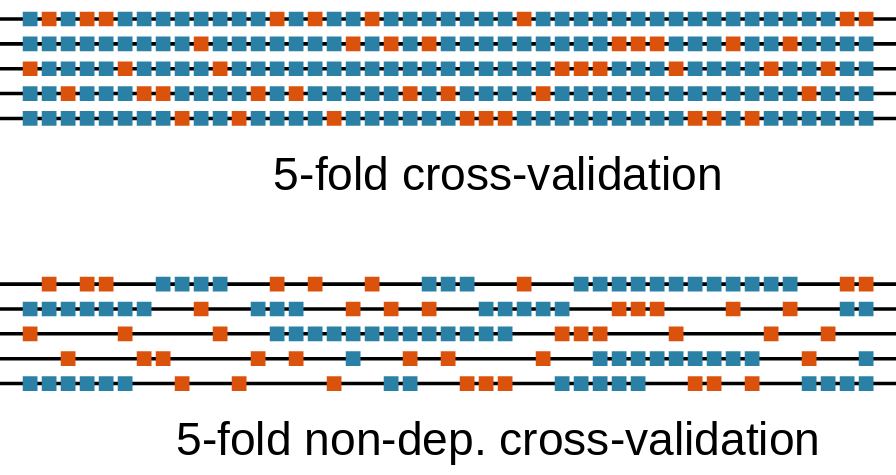
\includegraphics[width=0.9\linewidth]{Images/Cross-validation-scheme}
\caption{$\mathcal{K}$-fold CV and $\mathcal{K}$-fold with non-dependent data. Observations in blue are used to estimation and in orange for evaluation. Note that non-dependent data doesn't use all dataset in each fold.}
\label{fig:cross-validation-scheme}
\end{figure}

\end{frame}

\begin{frame}{Time-series Cross-Validation}

\begin{itemize}

\item
The CV score is given by the sum of the loss function for each fold.
The optimum value of \(t\) in this criteria is the one that minimizes
the CV score: \[
\theta^* = \text{argmin}_\theta CV(\theta) = \sum_{k \in \mathcal{K}} \sum_{\alpha \in A} L_\alpha(q).
\]
\item
To optimize CV function in \(\theta\), we use the Nelder-Mead
algorithm, which is a known and widely used algorithm for black-box
optimization.
\end{itemize}

\end{frame}

\section{Nonparametric model}\label{nonparametric-model}

\begin{frame}{Nonparametric model}

\[
\hat{Q}_{Y|X}(\alpha,\cdot)\quad\in\quad  \underset{q(\cdot)\in\mathcal{Q}}{\text{arg min}}\, L_\alpha(q) = \sum_{t\in T}\rho_{\alpha}(y_{t}-q(x_t)),
\]

\begin{itemize}
\item
On nonparametric models, \(q_\alpha\) belongs to a space of limited
second derivative function \(\mathcal{Q}\).
\item
The \(\alpha\)-quantile function is flexible enough to capture
nonlinearities on the quantile function.
\end{itemize}

\end{frame}

\begin{frame}{Nonparametric model - Formulation}


\begin{IEEEeqnarray*}{llr}
\min_{q_{j t},\varepsilon^+_{t}, \varepsilon_t^-, \xi_t} \sum_{j \in J} \sum_{t \in T'}\left(\alpha_j \varepsilon_{t j }^{+}+(1-\alpha_j)\varepsilon_{t j }^{-}\right) + \lambda \sum_{t \in T'}\xi_{t j } \span \span \nonumber \\
s.t. \qquad & \varepsilon_{t}^{+}-\varepsilon_{t j }^{-}=y_{t}-q_{t j }, & \forall t \in T',\forall j \in J,\\
& D^{1}_{t j }=\frac{q_{j t+1}-q_{j t}}{x_{t+1}-x_{t}}, 
& \qquad\forall t \in T',\forall j \in J,\\   
& D^{2}_{t j }:=\frac{\left(\frac{q_{j t+1}-q_{j t}}{x_{t+1}-x_{t}}\right)-\left(\frac{q_{j t}-q_{j t-1}}{x_{t}-x_{t-1}}\right)}{x_{t+1}-2x_{t} + x_{t-1}} \span\\
& \xi_{t j}\geq D^2_{t j }, & \qquad\forall t \in T',\forall j \in J,\\
& \xi_{t j}\geq-D^2_{t j}, & \qquad\forall t \in T',\forall j \in J,\\
& \varepsilon_{t j}^{+},\varepsilon_{t j}^{-}, \xi_{t j}\geq0, & \qquad\forall t \in T',\forall j \in J,\\
& q_{t j} \leq q_{t,j+1}, & \qquad \forall t \in T', \forall j \in J,\nonumber \\  
\end{IEEEeqnarray*}


\end{frame}

\begin{frame}{Nonparametric vs.~Linear Model}

\begin{itemize}

\item
The nonparametric approach is more flexible to capture
heteroscedasticity.
\end{itemize}

\begin{figure}
\centering
\begin{minipage}[t]{\linewidth}
\centering
\begin{minipage}[t]{0.45\linewidth}
\centering     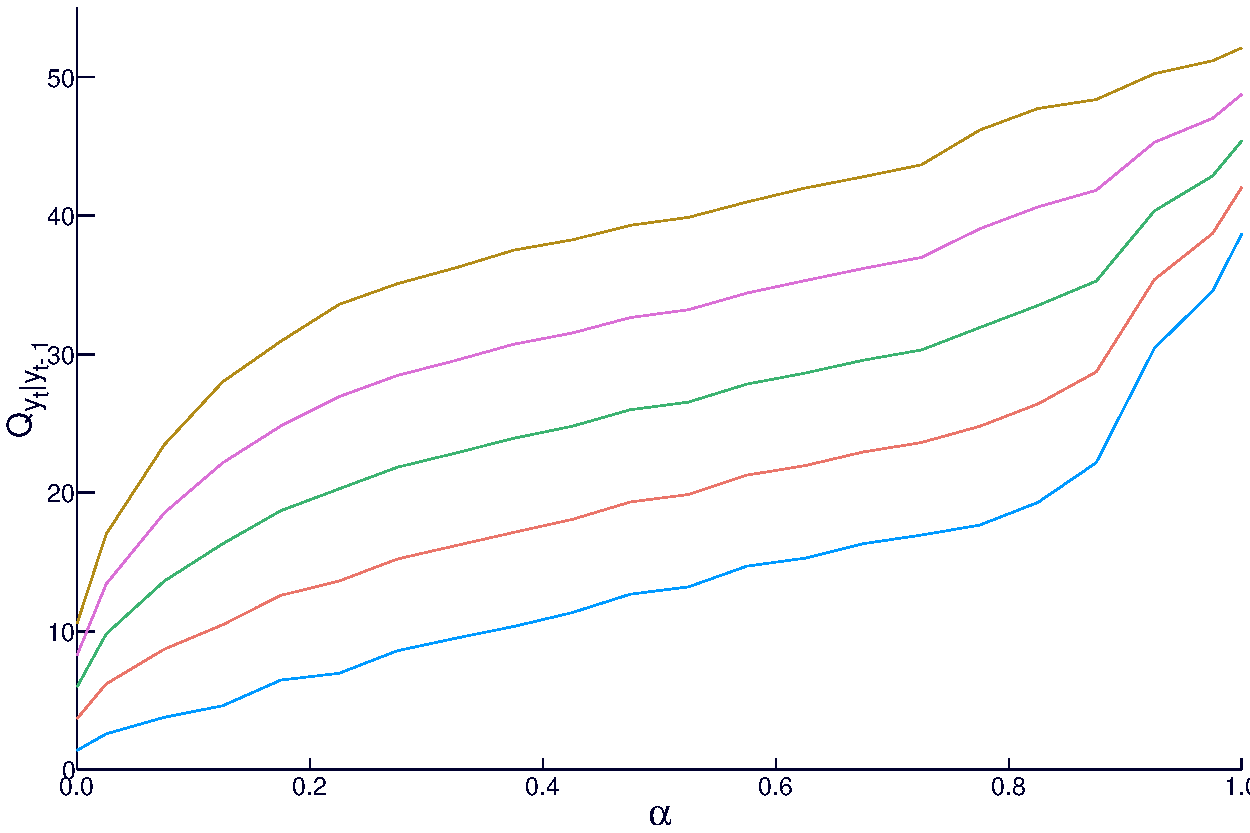
\includegraphics[width=\textwidth]{Images/icaraizinho-quantile-linear}
\end{minipage}
\begin{minipage}[t]{0.45\linewidth}
\centering     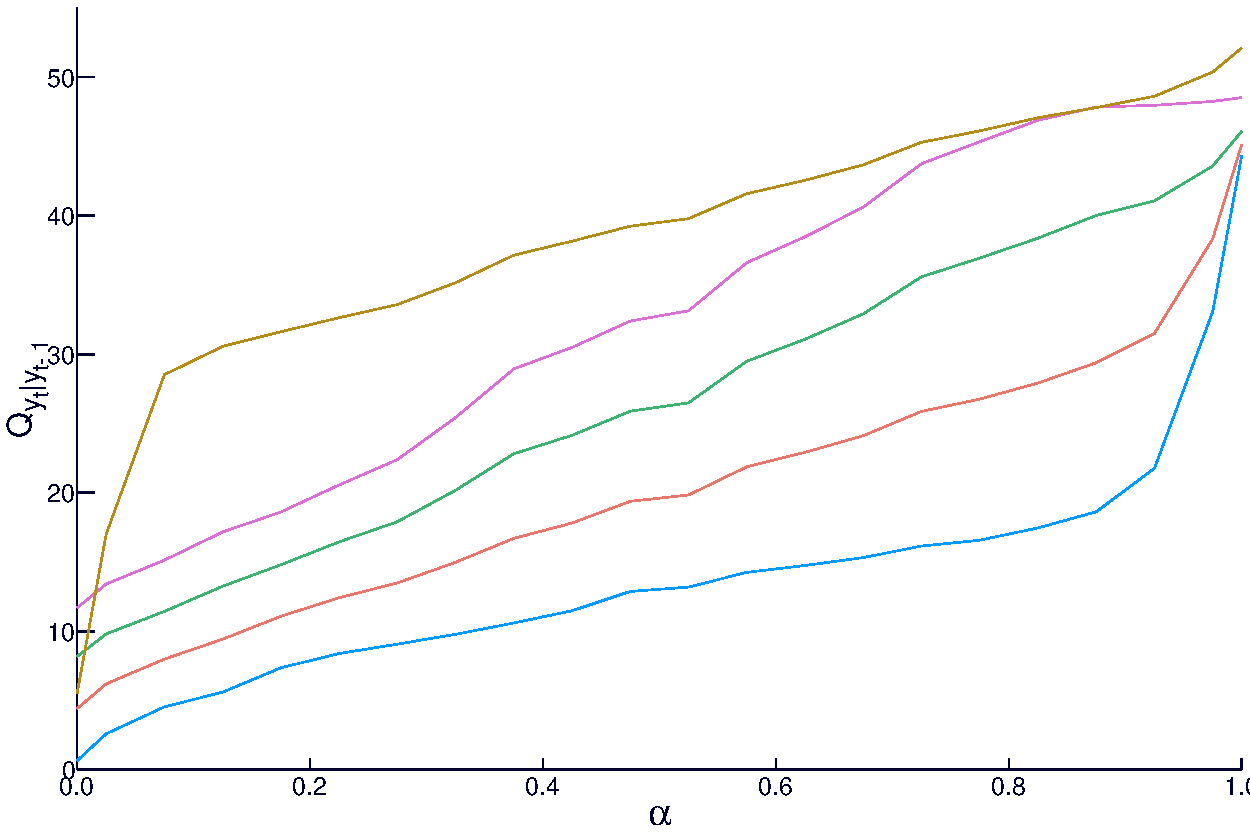
\includegraphics[width=\textwidth]{Images/icaraizinho-quantile-nonpar-lambda30}
\end{minipage}
\end{minipage}
\caption{Estimated quantile functions, for different values of $y_{t-1}$. On the left using a linear model and using a nonparametric approach on the right.}
\label{fig:quantiles-vs-xt}
\end{figure}

\end{frame}

\begin{frame}{Control of smoothing parameter}

\begin{itemize}

\item
This flexibility might lead to overfitting, if we don't select a
proper smoothing parameter.
\end{itemize}

\begin{figure}
\centering
\begin{minipage}[t]{\linewidth}
\centering
\begin{minipage}[t]{0.45\linewidth}
\centering     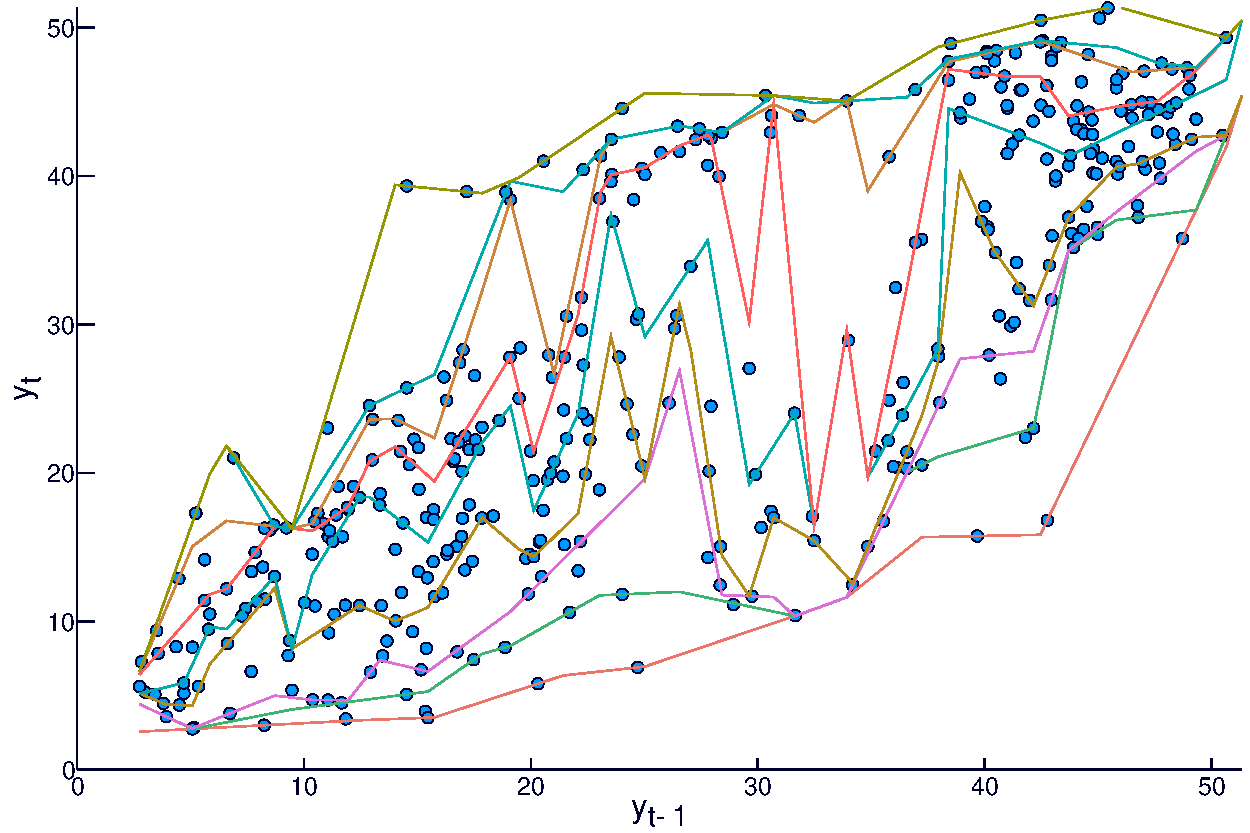
\includegraphics[width=\textwidth]{Images/icaraizinho-crossing-01}
\subcaption{$\lambda = 0.1$}
\end{minipage}
\begin{minipage}[t]{0.45\linewidth}
\centering     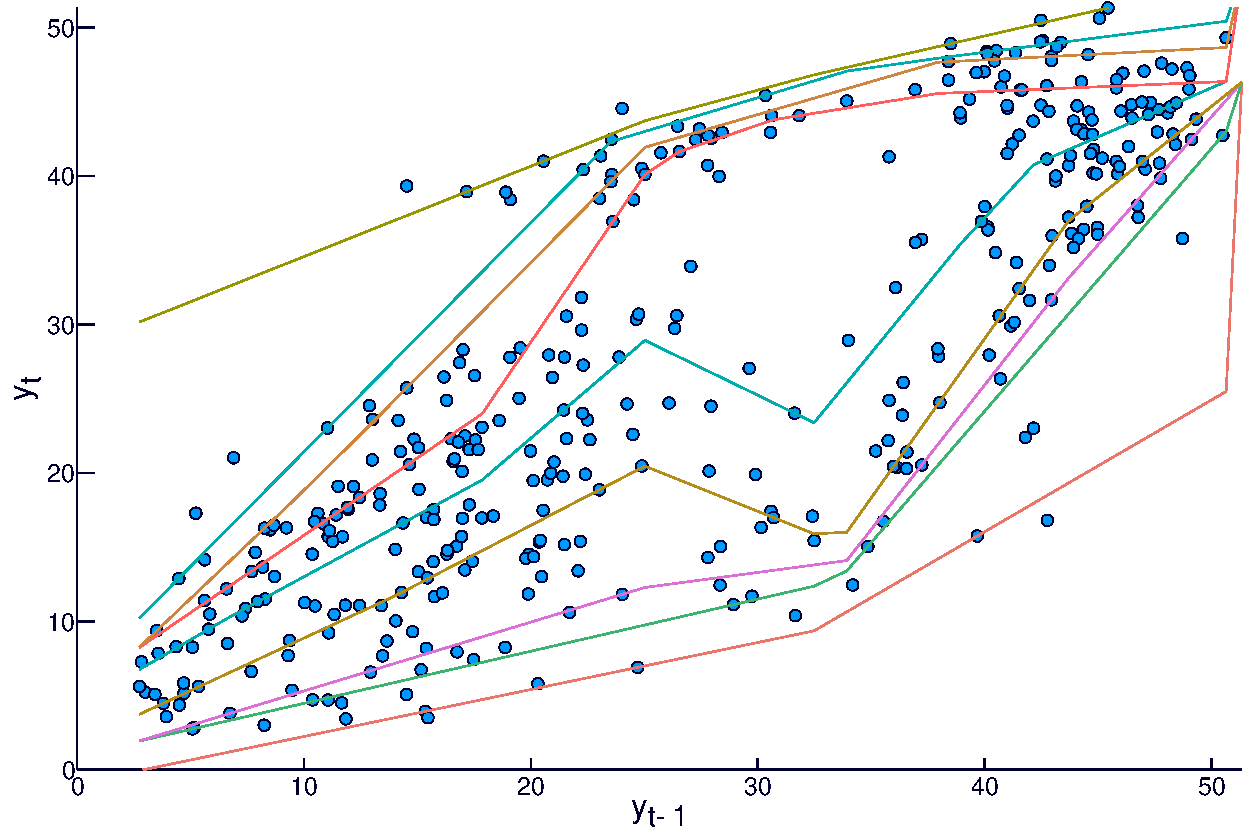
\includegraphics[width=\textwidth]{Images/icaraizinho-crossing-3}
\subcaption{$\lambda = 3$}
\end{minipage}
\end{minipage}
\end{figure}

\end{frame}

\begin{frame}{Control of smoothing parameter}

\begin{figure}
\centering
\begin{minipage}[t]{\linewidth}
\centering
\begin{minipage}[t]{0.45\linewidth}
\centering     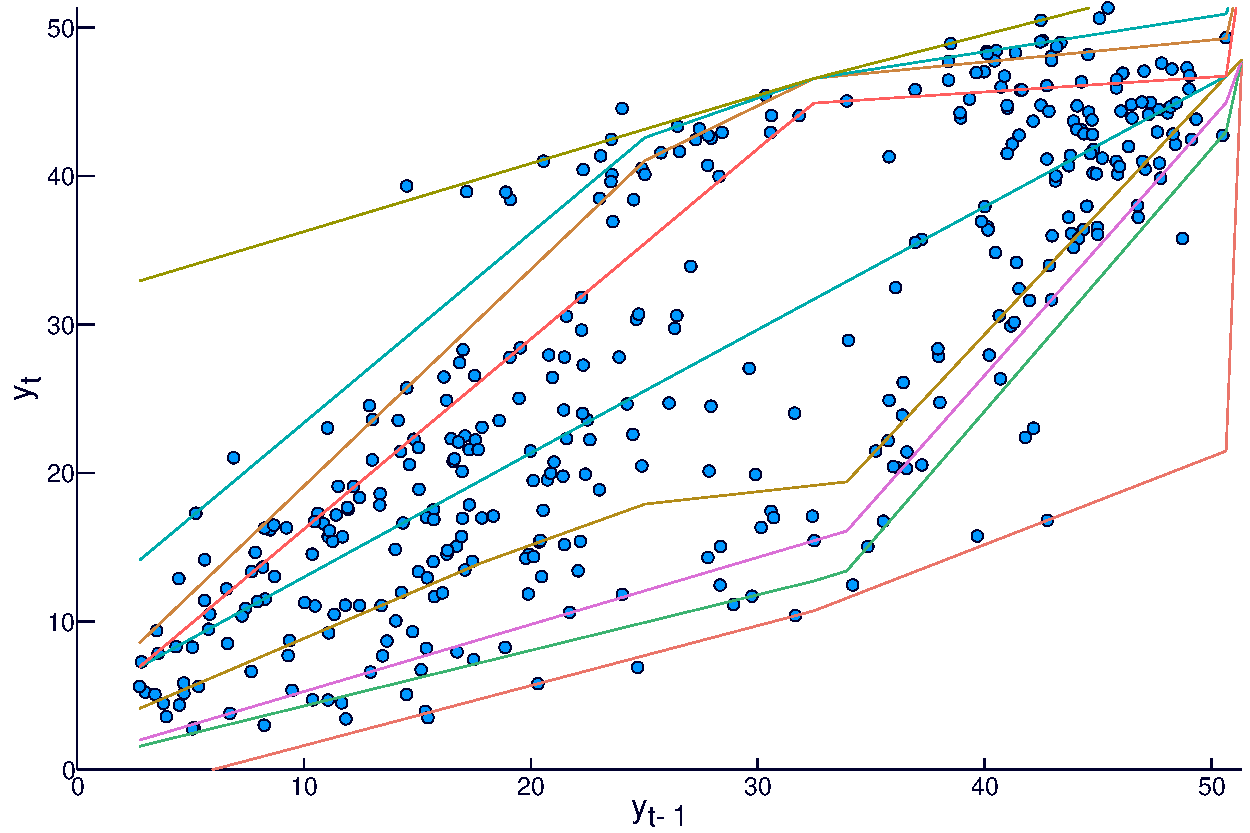
\includegraphics[width=\textwidth]{Images/icaraizinho-crossing-10}
\subcaption{$\lambda = 10$}
\end{minipage}
\begin{minipage}[t]{0.45\linewidth}
\centering     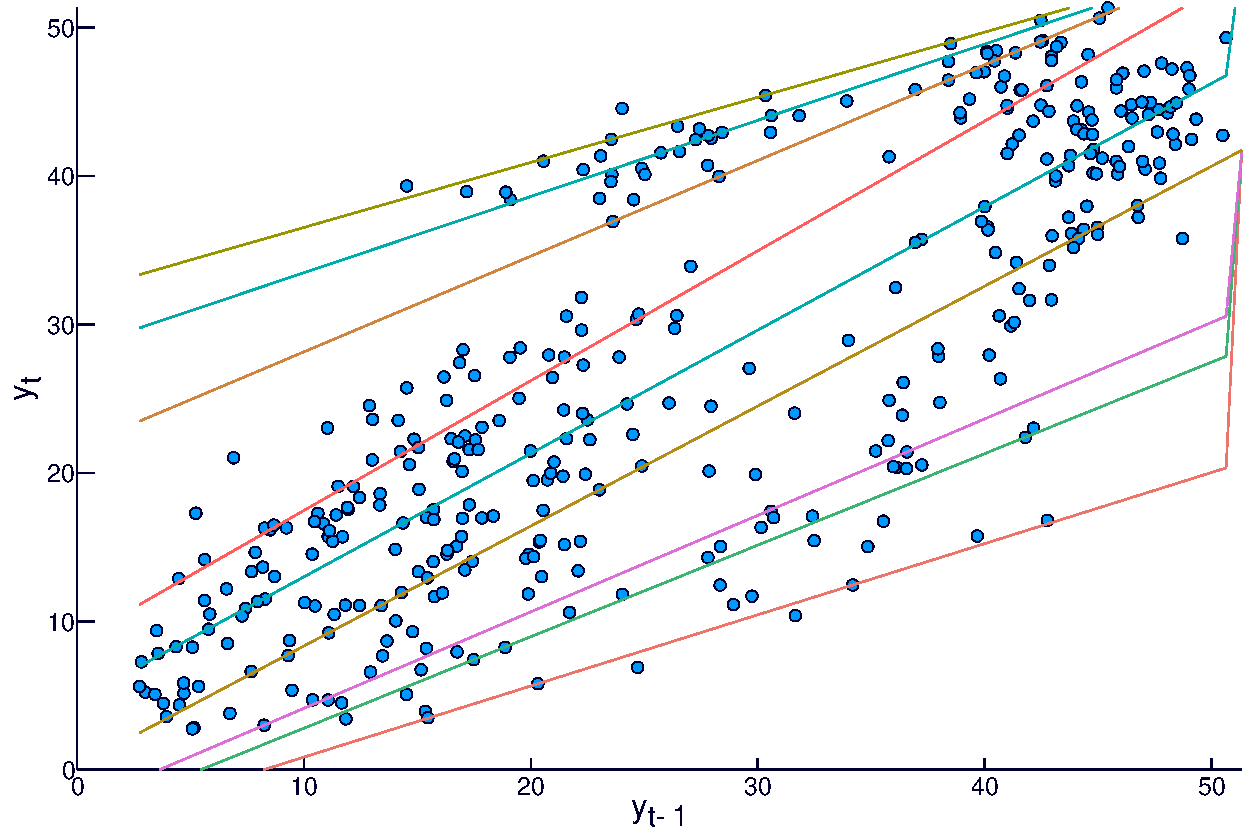
\includegraphics[width=\textwidth]{Images/icaraizinho-crossing-200}
\subcaption{$\lambda = 100$}
\end{minipage}
\end{minipage}
\end{figure}

\begin{itemize}

\item
On the limit, when \(\lambda \rightarrow \infty\), the nonparametric
model approaches a linear model.
\end{itemize}

\end{frame}

\begin{frame}{Present issues}

\begin{itemize}

\item
Difficult interpolation when \(x_t\) has dimension greater than 1.
\item
Control of smoothing parameter
\end{itemize}

\end{frame}

\section{Final}\label{final}


% Inserir slides com toda a bibliografia

\begin{frame}[allowframebreaks]
        \tiny
        \frametitle{References}
        \bibliographystyle{amsalpha}
          \bibliography{QR,Thesis,Bibhenriquinho}
\end{frame}

\end{document}
